\documentclass[journal]{IEEEtai}

\usepackage[colorlinks,urlcolor=blue,linkcolor=blue,citecolor=blue]{hyperref}

\usepackage{color,array}

\usepackage{graphicx}

\usepackage{soul}

\usepackage{makecell}
\usepackage{graphicx}
\usepackage{textcomp}
\usepackage{array} 
\usepackage{longtable}
\usepackage{booktabs}
\usepackage{float}

\usepackage{amsmath}
%% \jvol{XX}
%% \jnum{XX}
%% \paper{1234567}
%% \pubyear{2020}
%% \publisheddate{xxxx 00, 0000}
%% \currentdate{xxxx 00, 0000}
%% \doiinfo{TQE.2020.Doi Number}

\newtheorem{theorem}{Theorem}
\newtheorem{lemma}{Lemma}
\setcounter{page}{1}
%% \setcounter{secnumdepth}{0}


\begin{document}


\title{INT104 CW1-Lab report} 


\author{Ruiyang.Wu\quad	sID:2257475\quad E-Mail:Ruiyang.Wu22@student.xjtlu.edu.cn
	\\
	TA: Yu Kang \quad E-Mail:yu.kang23@student.xjtlu.edu.cn
}

\markboth{INT104 Artificial Intelligence CW1 2024/04/19 Ruiyang.Wu}
{INT104 Artificial Intelligence CW1 2024/04/19 Ruiyang.Wu}

\maketitle



\section{\textbf{Introduction}}

\IEEEPARstart{I}{n} this experiment, I first obtained the distribution state and correlation of the data through exploratory data analysis (EDA) of the raw data, and also used this as the basis for proposing hypotheses and proofs of the relationship between feature patterns and labels of some data. The raw data were then subjected to noise reduction and normalization to reduce the impact of noise and differences in data scale on subsequent operations. Then PCA dimensionality reduction was performed on the data as required, and by analyzing the distribution of the data on different feature vectors, the combination of vectors that best distinguished the original dataset was found, and the hypotheses proposed in the data observation were also verified. Finally I used my own way of extracting features from the raw dataset and comparing them with each of the previous features to each other. \textbf{To ensure reproducibility of the experiments}, the code for this paper has been placed in a GitHub repository:  
\href{https://github.com/MushihimePepsi/XJTLU_ICS_Y2S2_Course-notes_23-24/tree/main}{\ul{https://github.com/MushihimePepsi/XJTLU\_ICS\_Y2S2\_Course-notes\_23-24/tree/main}}


\section{\textbf{Task1-Data Observation, Cleaning \& Normalization}}

There were a total of 619 samples in the raw dataset with no missing or incorrectly recorded data. Each tuple included the student's index, gender, grade, major (as label), and scores. To eliminate the effects of data scales and outliers on the analysis, the raw data were first standardized using Z-Score before plotting box plots based on different majors [Fig. 1]. I found that all Programme3 students belonged to grade3, while only a few students in other majors belonged to grade3. \textbf{Conjecture that Programme3 could be separated first based on the features of grades}. Furthermore, \textbf{in 'MCQ', 'Q1 ', 'Q4' features, the distribution of different majors varies greatly}, which may serve as potential separation features.

\begin{figure}[htbp]
\centerline{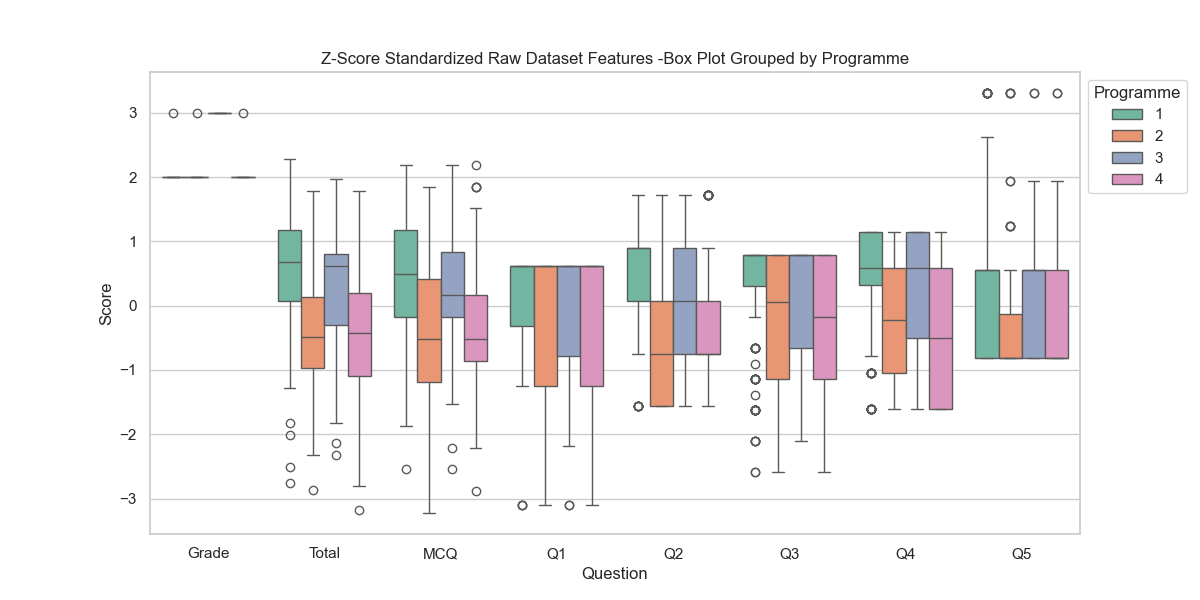
\includegraphics[width=22pc]{Z-Score_raw_dataset_box_plot_by_programme.png}}
\caption{standardized box plots grouped by 'Programme'(analysis distribution)}
\end{figure}

Since many statistical methods are not applicable to non-normally distributed data, normality test is required for continuous type variables. Due to small sample size(\textless 2000), Shapiro-Wilk test was used here and all the variables were found to have p-value far less than 0.01 [Fig. 2] and \textbf{were not Gaussian distributed}.

\begin{figure}[htbp]
	\centerline{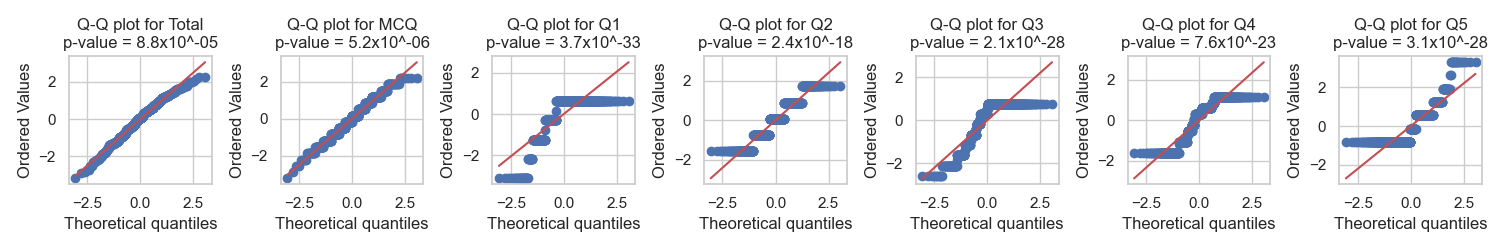
\includegraphics[width=22pc]{Shapiro-Wilk test.png}}
	\caption{Q-Q plot and p-value (Shapiro-Wilk test) of each feature}
\end{figure}

Due to the non-normal distribution of the data, I explored the monotonic correlation between features using the Spearman correlation coefficient instead of the Pearson correlation coefficient. It can be found that in the correlation between features, \textbf{'gender' and 'grade' have very little monotonic correlation with the score items ('Total'~ 'Q5')}; while the \textbf{high monotonic correlation of 'Total' with other score features} is due to the fact that it comes from a \textbf{linear combination} of the scores. Therefore, 'Total' can be considered to remove from the feature set.

\begin{figure}[htbp]
	\centerline{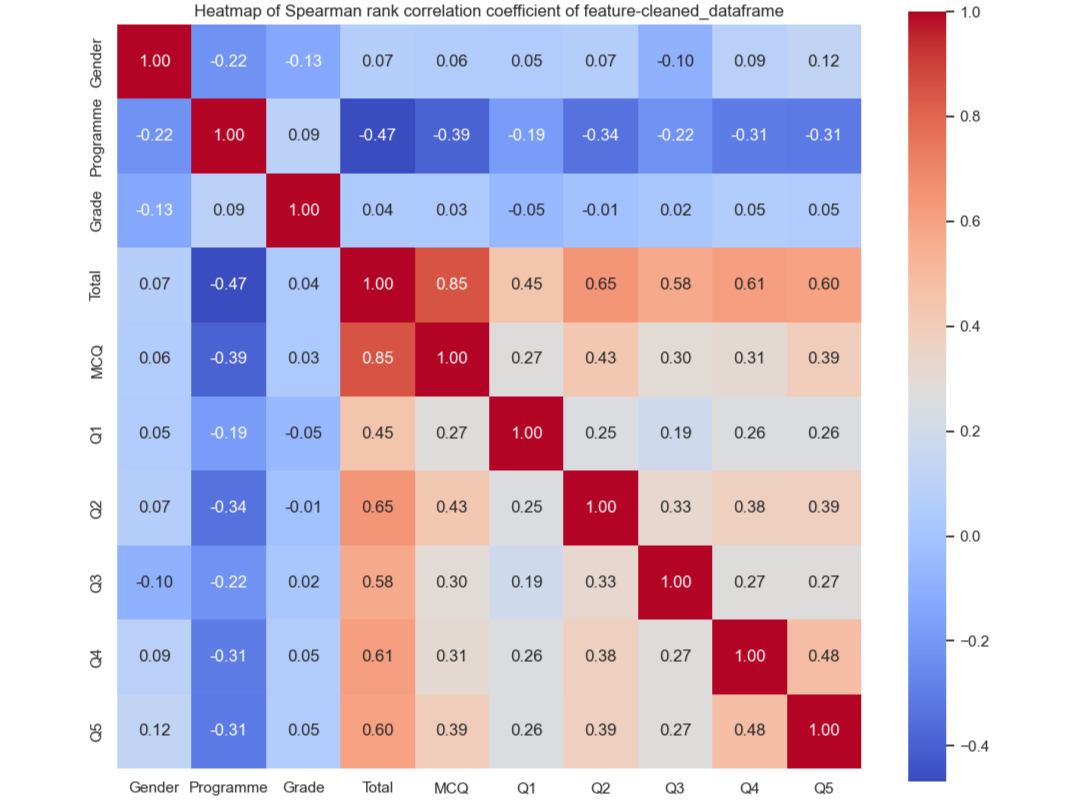
\includegraphics[width=20pc]{spearman_corr_features.png}}
	\caption{Spearman correlation between features}
\end{figure}

Due to the nonlinear relationship between features and labels, I used the maximum mutual information coefficient (MIC), which is based on information entropy, to measure the degree of correlation between each feature and Programme. It can be found that Grade has the greatest correlation with major, which is caused by the fact that \textbf{all Programme3 students are grade3}. Whereas, the MIC of 'Gender' is extremely low, so it \textbf{can be considered to be removed from the feature set}. Also, the larger MICs for 'MCQ', 'Q1', and 'Q4' \textbf{validate the earlier conjecture that they may serve as separating features}.

\renewcommand\arraystretch{1.5}%保证每列高度是原先的1.5倍
\begin{table}[htbp]%星号表示双栏
	\caption{MIC between label and each feature}
	\begin{tabular}{p{0.5cm}<{\centering}p{0.5cm}<{\centering}p{0.5cm}<{\centering}p{0.5cm}<{\centering}p{0.5cm}<{\centering}p{0.5cm}<{\centering}p{0.5cm}<{\centering}p{0.5cm}<{\centering}p{0.7cm}<{\centering}}%设定每列的宽度以及对齐方式,并且可以做到自动换行
		\Xhline{1.2pt}%第一条粗线
		\textbf{Grade} & \textbf{Total} & \textbf{MCQ} & \textbf{Q2} & \textbf{Q4} & \textbf{Q5} & \textbf{Q3} & \textbf{Q1} & \textbf{Gender} \\ 
		\Xhline{1.2pt}%第二条粗线
		0.280 & 0.252 & 0.147 & 0.128 & 0.106 & 0.100 & 0.084 & 0.068 & 0.047 \\ 
		\Xhline{1.2pt}%第三条粗线
	\end{tabular}
	\label{MRFsum}
\end{table}


\section{\textbf{Task2-PCA dimensional reduction}}
Based on the above conclusions, I select seven features ['Grade','MCQ','Q1','Q2','Q3','Q4','Q5'] as inputs for Principal Components Analysis (PCA) dimensionality reduction, and the two feature vectors explaining the largest variance ratios are selected as the direction of dimensionality reduction. With 54.4\%[Fig. 5] of the total variance explained in these two directions which can \textbf{separate Programme3 well} in principle component 2, and it can \textbf{also be found that the samples of Programme1 tend to be in the negative half-axis of principle component 1 while the samples of Programme4 tend to be in the positive half-axis of it} [Fig. 4].

\begin{figure}[htbp]
	\centerline{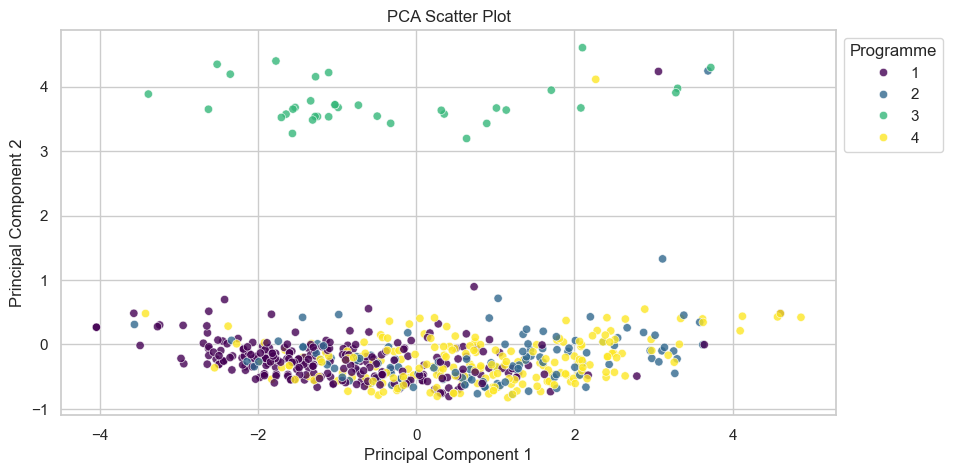
\includegraphics[width=22pc]{pca_7_features_in.png}}
	\caption{PCA input=[Grade,MCQ,Q1,Q2,Q3,Q4,Q5] largest 2 eigenvectors}
\end{figure}

\begin{figure}[htbp]
	\centerline{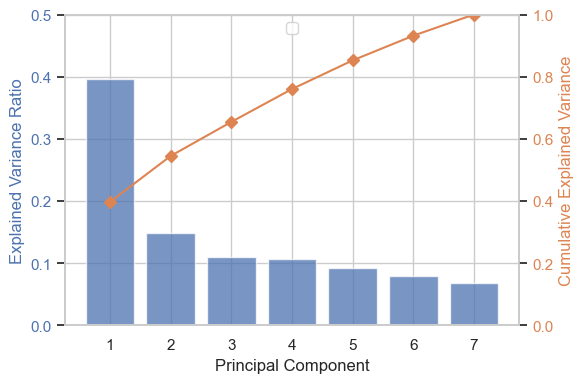
\includegraphics[width=20pc]{pca_7_features_acc_in_6-4.png}}
	\caption{Explained Variance Ratio \& Cumulative Explained Variance}
\end{figure}

\section{\textbf{Task3-It's MyGo to find resulting features}}
The correspondence between Grade=3 and Programme=3 can be statistically derived. In the dataset, Grade=3 was used as a predictor for predicting Programme=3:

\begin{table}[htbp]  
	\caption{Predicting 'Programme'=3 with feature 'Grade'=3} % 添加表格标题 
	\centering % 将表格居中显示  
	\begin{tabular}{|c|c|c|}  
		\hline  
		\textit{Confusion Matrix} & \textbf{True Programme=3} & \textbf{True Programme$\neq$3} \\ \hline  
		\textbf{Pred. Programme=3} & TP=35 & FP=3 \\ \hline  
		\textbf{Pred. Programme$\neq$3} & FN=0 & TN=581 \\ \hline  
	\end{tabular}   
\end{table}

\renewcommand\arraystretch{1.5}%保证每列高度是原先的1.5倍
\begin{table}[htbp]%星号表示双栏
	\caption{Performance of the classification by 'Grade'}
	\begin{tabular}{p{1.7cm}<{\centering}p{1.7cm}<{\centering}p{1.7cm}<{\centering}p{1.7cm}<{\centering}p{1.7cm}<{\centering}}%设定每列的宽度以及对齐方式,并且可以做到自动换行
		\Xhline{1.2pt}%第一条粗线
		\textbf{Precision} & \textbf{Recall} & \textbf{Accuracy} & \textbf{F1 Score}  \\ 
		\Xhline{1.2pt}%第二条粗线
		92.11\% & 100\% & 99.52\% & 95.89\% \\ 
		\Xhline{1.2pt}%第三条粗线
	\end{tabular}
	\label{MRFsum}
\end{table}

The performance of this classification is satisfactory. So we can \textbf{remove the feature 'Grade'} (the rest of the samples all belong to 'Grade' = 2). My subsequent feature extraction will focus on finding the feature space that separates Programme={1,2,3}. I remove the Grade features and also remove the samples with Grade=3 from the dataset and \textbf{delete the outliers in the dataset by Isolation Forests}, then the \textbf{input features are ['MCQ', 'Q1', 'Q2', 'Q3', 'Q4', 'Q5']} and there exist 400 samples (as visualized by t-SNE [Fig. 6]) It can be found that \textbf{the Programme1 and 4 have tendency of different distributions}.

\begin{figure}[htbp]
	\centerline{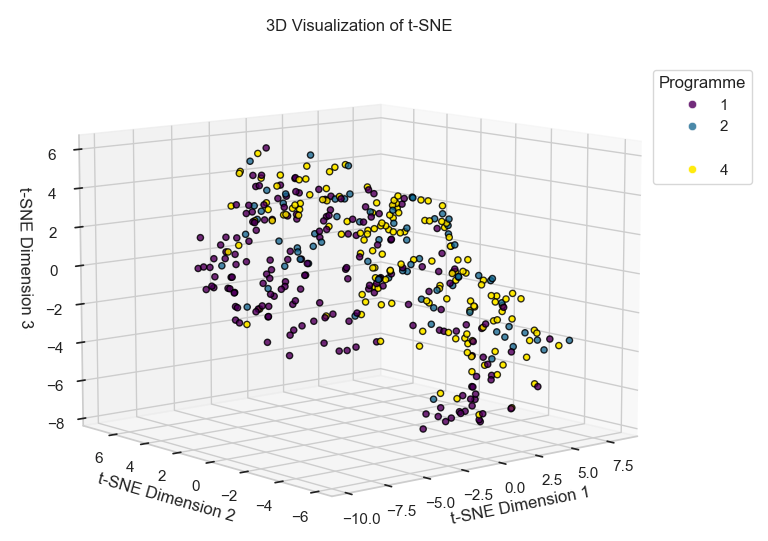
\includegraphics[width=22pc]{tsne_3_dazim=230_mod.png}}
	\caption{My chosen feature space visualized via t-SNE}
\end{figure}

After comparing various dimensionality reduction methods, I finally used Kernel Principal Component Analysis (KPCA) in the case of t-distributed Stochastic Neighbor Embedding (t-SNE) (which reduced the original feature space to three dimensions) in an attempt to find the high-dimensional feature vector which maximizes the variance of the sample points to separate them. I used polynomial function [Fig.7] or Radial Basis Function (RBF) [Fig.8] as kernel function and performed parameter optimization to get the resulting features, it can be found that the two-dimensional feature distinguishes Programme1 and 4 more clearly, but classifies Programme2 poorly [Fig.7].This is the result of purely unsupervised learning, which already gives a two-dimensional feature space that tends to be approximately linearly divisible, with the features of new feature space coming from the nonlinear combination of the raw features.

\begin{figure}[htbp]
	\centerline{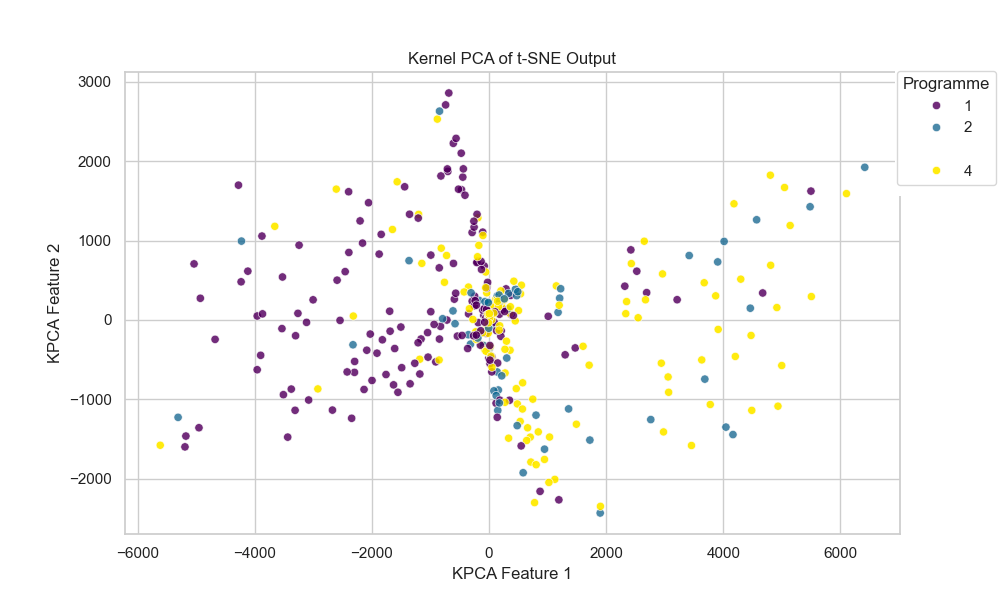
\includegraphics[width=22pc]{kpca_after_tnse2d_poly_mod.png}}
	\caption{KPCA using polynomials as kernel function}
\end{figure}

\begin{figure}[htbp]
	\centerline{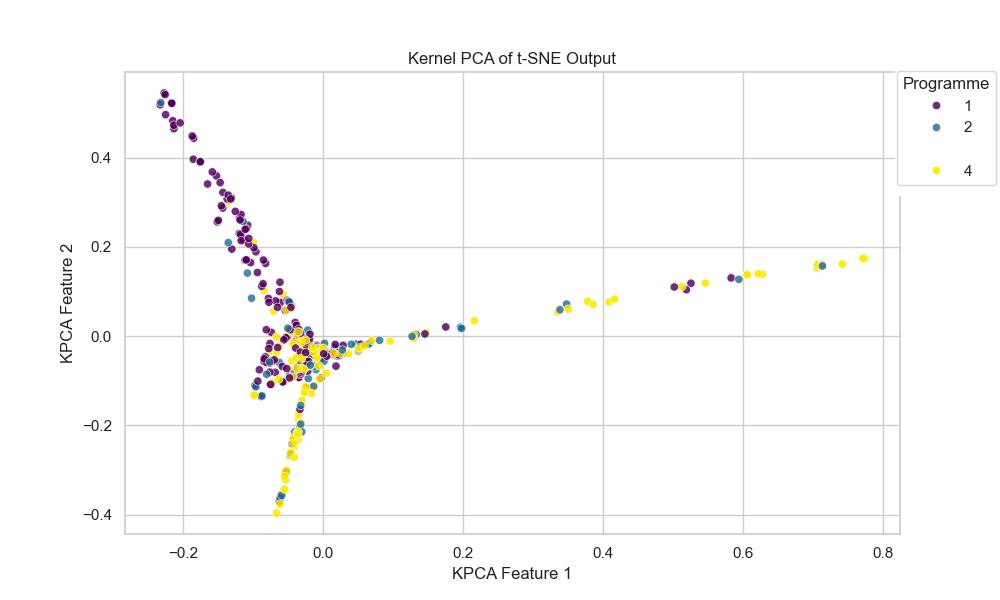
\includegraphics[width=22pc]{kpca_after_tnse2d_rbf_mod.png}}
	\caption{KPCA using RBF as kernel function (optimized)}
\end{figure}


\section{\textbf{Task4-Conclusion \& Critical thinking}}
\subsection{Summary of the proposal of scientific hypotheses and proofs}
In this experiment, \textbf{hypotheses are proposed and proved} to characterize the distribution patterns of several features and labels through exploratory data analysis of the original data. The correspondence between Programme3 and Grade3 is proved and used to reduce the dimensionality; the 'MCQ', 'Q1', and 'Q4' features are proved to be highly correlated to the 'Programme' and they are chosen as potential separation features; demonstrating the irrelevance of 'Gender' and using this to reduce dimensionality; and demonstrating that the high correlation between 'Total' and other scores is due to the fact that 'Total' comes from a linear combination of other scores and using this to reduce dimensionality.

\subsection{Summary of comparison of raw /scaled /PCA /my resulting features}
Relative to the original features, the scaled feature removes the effect of scale and appropriately removes low correlation or redundant features (Gender, Total) through statistical manipulation.The PCA feature finds a way to categorize Programme3 by transforming the coordinate system. My features went a step further by noise-reducing the data, attempting to reduce the feature space of the data to two dimensions through a combination of manifold learning and kernel functions.

\subsection{Critical Thinking and Current Shortcomings}
In my resulting features, the classification of 'Programme'=2 was poor. To solve this problem, I conjecture that nonlinear dimensionality reduction methods based on supervised learning should be used, such as combining Linear Discriminant Analysis (LDA) with kernel functions to find features of the sample points that differentiate between different LABELS, rather than features that maximize the variance of the sample. I also conjecture that the feature space that maximizes the ability to distinguish students' majors will come from a nonlinear combination of the original features.

\subsection{Statement of my final feature selection}
Overall, I will choose ['Grade', 'MCQ', 'Q1', 'Q2', 'Q3', 'Q4', 'Q5'] as the features for subsequent classification. I discarded 'Gender' due to the low relevance of this feature for categorization (MIC); removing 'Total' due to the fact that this feature can be obtained from a linear combination of other features. I kept 'Grade', due to the strong correlation demonstrated above, which can be used to categorize Programme3 by this feature; and keeping the rest of the scores, as they still show a strong correlation to labels.


\section{\textbf{Acknowledgment}}
I would like to thank the two TAs of SC375: Yu Kang and Yiqiang Cai for their detailed comments and guidance.

I would like to thank Dr. Shengchen Li for his careful design of the experiments in this course and his discussions with me in the classroom, which helped me to gain a deeper understanding of traditional machine learning, as well as an interest in the study of artificial intelligence. Thanks to Dr. Liu and Dr. Kang for their lectures and accepting me to participate in Dr. Liu's research.





\end{document}
